\documentclass[11pt]{article}

\newcommand{\cnum}{ECE M146}
\newcommand{\ced}{Spring 2023}
\newcommand{\ctitle}[4]{\title{\vspace{-0.5in}\cnum, \ced\\Homework Set #1: #2}\author{\vspace{-0.35in}\\Name: #3, UID: #4}}
\usepackage{enumitem}
\newcommand{\solution}[1]{{{\color{blue}{\bf Solution:} {#1}}}}
\usepackage[usenames,dvipsnames,svgnames,table,hyperref]{xcolor}
\usepackage{amsmath, amsfonts}
\usepackage{graphicx} % Required for inserting images
\usepackage{float}
\usepackage{listings}
\usepackage{xcolor}
\usepackage{hyperref}

\renewcommand*{\theenumi}{\alph{enumi}}
\renewcommand*\labelenumi{(\theenumi)}
\renewcommand*{\theenumii}{\roman{enumii}}
\renewcommand*\labelenumii{\theenumii.}

\definecolor{codegreen}{rgb}{0,0.6,0}
\definecolor{codegray}{rgb}{0.5,0.5,0.5}
\definecolor{codepurple}{rgb}{0.58,0,0.82}
\definecolor{backcolour}{rgb}{0.95,0.95,0.92}

\lstdefinestyle{mystyle}{
    backgroundcolor=\color{backcolour},
    commentstyle=\color{codegreen},
    keywordstyle=\color{magenta},
    numberstyle=\tiny\color{codegray},
    stringstyle=\color{codepurple},
    basicstyle=\ttfamily\footnotesize,
    breakatwhitespace=false,
    breaklines=true,
    captionpos=b,
    keepspaces=true,
    numbers=left,
    numbersep=5pt,
    showspaces=false,
    showstringspaces=false,
    showtabs=false,
    tabsize=2
}


\begin{document}
\ctitle{\#0}{}{Asher Christian}{006-150-286}
\date{}
\maketitle
\vspace{-0.75in}
\section{Problem 1}
Consider $y = x\sin(z)e^{-x}$ what is the partial of $y$ with respect to $x$?\\
\solution{
\[
    \frac{\partial y}{\partial x} = \sin(z)e^{-x} - x\sin(z)e^{-x}
.\] 
}

\section{Problem 2}
Consider the matrix $X$ and the vectors $y$ and $z$ below:
\[
    X = \begin{pmatrix} 2 & 4 \\ 1 & 3 \end{pmatrix} \hspace{1cm} y = \begin{pmatrix} 1 \\ 3 \end{pmatrix} \hspace{1cm} z = \begin{pmatrix} 2 \\ 3 \end{pmatrix} 
.\] 
\begin{enumerate}
    \item What is the inner product $y^{T}z$?
    \item What is the product $Xy$?
    \item is $X$ invertible? If so, give the inverse; if not, explain why not.
    \item What is the rank of $X$?
\end{enumerate}
\solution{
   \begin{enumerate}
       \item
           \[
           y^{T}z = 1\cdot 2 + 3 \cdot 3 = 11
           .\] 
       \item
           \[
           Xy = \begin{pmatrix} 2 \cdot 1 + 4 \cdot 3 \\ 1 \cdot 1 + 3 \cdot 3 \end{pmatrix}  = \begin{pmatrix} 14 \\ 10 \end{pmatrix} 
           .\] 
       \item 
           \[
           \det(X) = 6 -4 = 2 \ne 0
           .\] 
           yes $X$ is invertible inverse given by formula for $X \in \mathbb{R}^{2 \times 2}$
           \[
               X^{-1} = \frac{1}{2}\begin{pmatrix} 3 & -4 \\ -1 & 2 \end{pmatrix}  = \begin{pmatrix} 1.5 & -2 \\ -.5 & 1 \end{pmatrix} 
           .\] 
       \item Since $X$ is invertible its rank is equal to its domain and range which is 2
   \end{enumerate} 
}
\section{Problem 3}
Consider a sample of data $S$ obtained by flipping a coin five times. $X_i, i \in \{1,...,5\}$ is a random 
variable that takes a value 0 when the outcome of coin flilp  $i$ turned up heads, and 1 when it turned up tails.
Assume that the outcome of each of the flips does not depend on the outcomes of any other flips.
The sample obtained $S = (X_1,X_2,X_3,X_4,X_5) = (1,1,0,1,0)$
\begin{enumerate}
    \item What is the sample mean for this data?
    \item What is the unbiased sample variance?
    \item What is the probability of observing this data assuming that a coin with
        and equal probability of heads and tails was used?
    \item Note the probability of this data sample would be greater if the value 
        of the probability of tails $P(X_i = 1)$ was not $0.5$ but some other value. What is the value that maximizes the
        probability of the sample $S$? Can you prove your answer is corret?
    \item Given the following joint distribution between $X$ and $Y$ what is $P(X=T|Y=b)$
\end{enumerate}
\solution{
    \begin{enumerate}
        \item sample mean
            \[
            \mu =\frac{1}{5}(1 + 1 + 0 + 1 + 0) = \frac{3}{5} = 0.6
            .\] 
        \item sample unbiased variance
            \[
            s^2 = \frac{0.4^2 + 0.4^2 + 0.6^2 + 0.4^2 + 0.6^2}{5-1} = 0.3
            .\] 
            \[
            s = \sqrt{s^2} \approx 0.548
            .\] 
        \item 
            $P(S) = \frac{1}{2}^{5} \approx 0.031$ 
        \item 
            The probability would be maximized by taking $p =P(X_i = 1) = 0.6$
            This can be seen by finding the value  $p$ maximizing the joint distribution
            the probability mass function of each $X_i$ is $P(X_i = x) = p^{x}(1-p)^{(1-x)}$
            the joint distribution $P(S:p) = p^{\sum_{}^{}x_i}(1-p)^{n-\sum_{}^{}x_i}$ 
            To maximize this probability over $p$ we can maximize its log likelihood
            \[
            \ln(P(S:p)) = (\sum_{}^{}x_i)\ln(p) + (n-\sum_{}^{}x_i)\ln(1-p)
            .\] 
            \[
                \frac{d\ln(P(S:p))}{dp} = \frac{\sum_{}^{}x_i}{p}-\frac{n-\sum_{}^{}x_i}{1-p} = 0
            .\] 
            \[
            0 = (1-p)\sum_{}^{}x_i - np + p\sum_{}^{}x_i = \sum_{}^{}x_i -np
            .\]  
            \[
            np = \sum_{}^{}x_i \implies p = \mu
            .\] 
            thus setting  $p = \mu $ maximizes the joint probability distribution of the data.
        \item 
            $P(X=T|Y=b) = \frac{0.1}{0.1+0.15} = .4$
    \end{enumerate}
}

\section{Problem 4}
math the distribution to its formula
\solution{
    \begin{align*}
        (a) &= (v) = \frac{1}{\sqrt{(2\pi)\sigma^2}}e^{-\frac{1}{2\sigma^2}(x-\mu)^2}\\
        (b) &= (iv) = \lambda e^{-\lambda x}\\
        (c) &= (ii) = \frac{1}{b-a}\\
        (d) &= (i) = p^{x}(1-p)^{1-x}\\
        (e) &= (iii) = \binom{n}{x}p^{x}(1-p)^{n-x}\\
    \end{align*}
}

\section{Problem 5}
\solution{
    \begin{enumerate}
        \item $X \sim \text{Bernoulli}(s)$ then $E[X] = 1\cdot p^{1}(1-p)^{1-1} + 0\cdot p^{0}(1-p)^{1-0} = p = \mu$ 
            For variance $E[(X-\mu)^2] = (1-p)^2p + (0-p)^2(1-p) = p(1-p)(1-p +p) = p(1-p)$ 
        \item variance of $2X$ is $4\sigma^2$ variance of $X+2$ is still $\sigma^2$
    \end{enumerate}
}

\section{Problem 6}
\solution{
    \begin{enumerate}
        \item $lg(n) = \frac{\ln(n)}{\ln(2)}$ so $f(n) = \ln(2)g(n)$ and $g(n) = \frac{f(n)}{\ln(2)}$ and so $f(n) = O(g(n))$ and $g(n) = O(f(n))$ 
        \item $g(n) = O(f(n))$ but not vice versa. Taking derivatives makes it obvious that $\ln(3)3^{n} \gg 10n$ 
        \item 
            \[
            3^{n} = 2^{lg(3)n}
            .\] 
            so clearly $g(n) = O(f(n))$ however assume for contradiction there exists $M$ such that
            \[
            3^{n} < M 2^{N}
            .\] 
            for all $n > N$ then
             \[
                 (\frac{3}{2})^{n} < M
            .\] 
            however $\frac{3}{2} > 1$ so $\frac{3}{2}^{n}$ grows exponentially a contradiction thus $3^{n} \ne O(2^{n})$
    \end{enumerate}
}

\section{Problem 7}
if $X$ and $Y$ are independent random variables, show that $\mathbb{E}[XY] = \mathbb{E}[X] \mathbb{E}[Y]$
\solution{
   if $XY$ has joint pdf $f(x,y)$
   \[
       \mathbb{E}[XY] = \int_{}^{}\int_{}^{}f(x,y)dxdy = \int_{}^{}\int_{}^{}f(x)_Xf(y)_Ydxdy = \int_{}^{}f(x)_Xdx\int_{}^{}f(y)_Ydy = \mathbb{E}[X] \mathbb{E}[Y]
   .\] 
   with the last step being that
   \[
   f(x,y) = f(x)_X f(y)_Y
   .\] 
   by independence.
}
\section{Problem 8}
\solution{
    \begin{enumerate}
        \item 
        \begin{enumerate}
            \item unit sphere centered at the origin (radius 1)
                \begin{figure}[h]
                    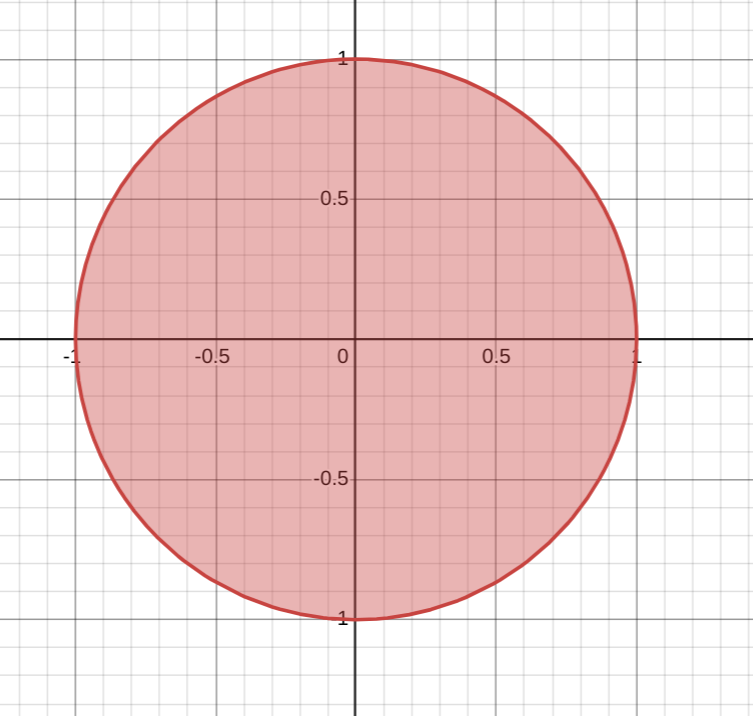
\includegraphics[width=0.3\textwidth]{unit_sphere.png} 
                \end{figure}
            \item line $x=0$ and line $y=0$ including the origin.
                \begin{figure}[h]
                    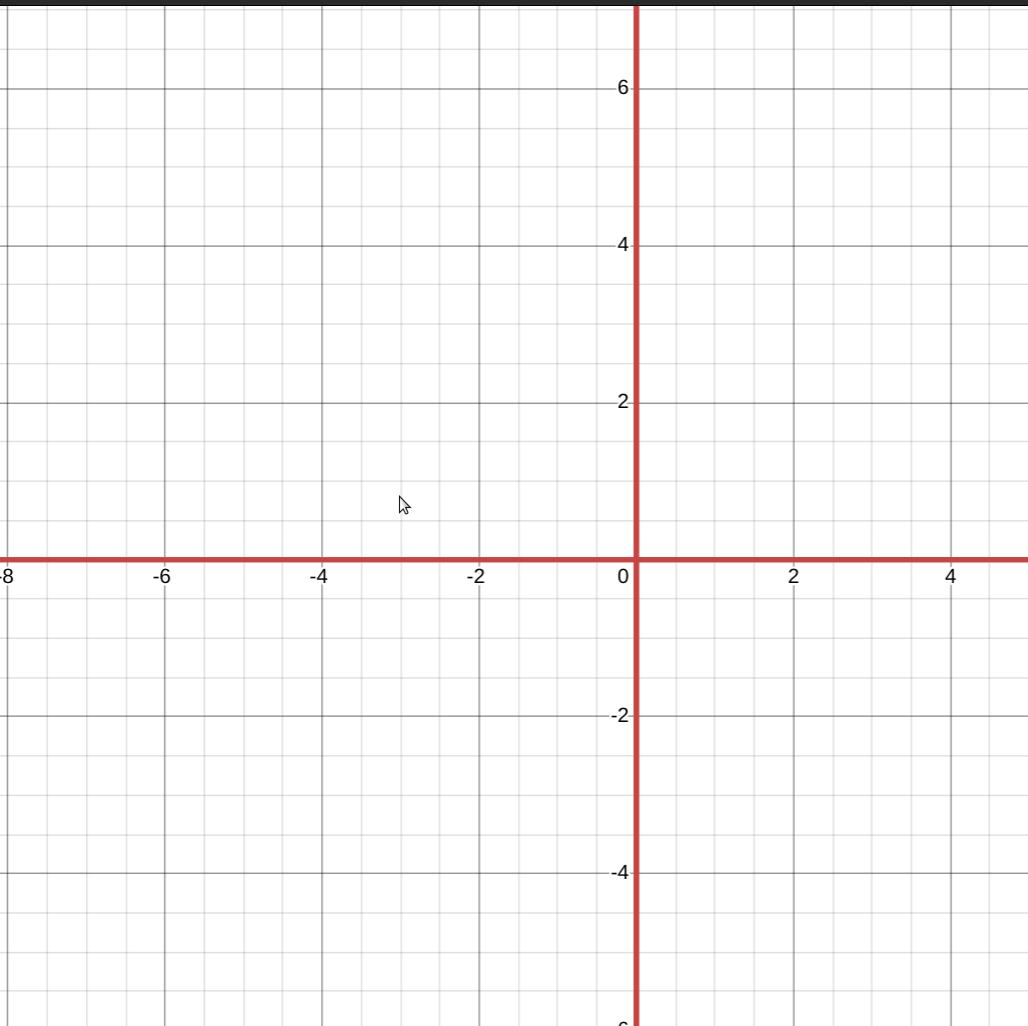
\includegraphics[width=0.3\textwidth]{lines.png}                
                \end{figure}
            \item half square centered at origin (radius 1) rotated 45 degrees
                \begin{figure}[h]
                    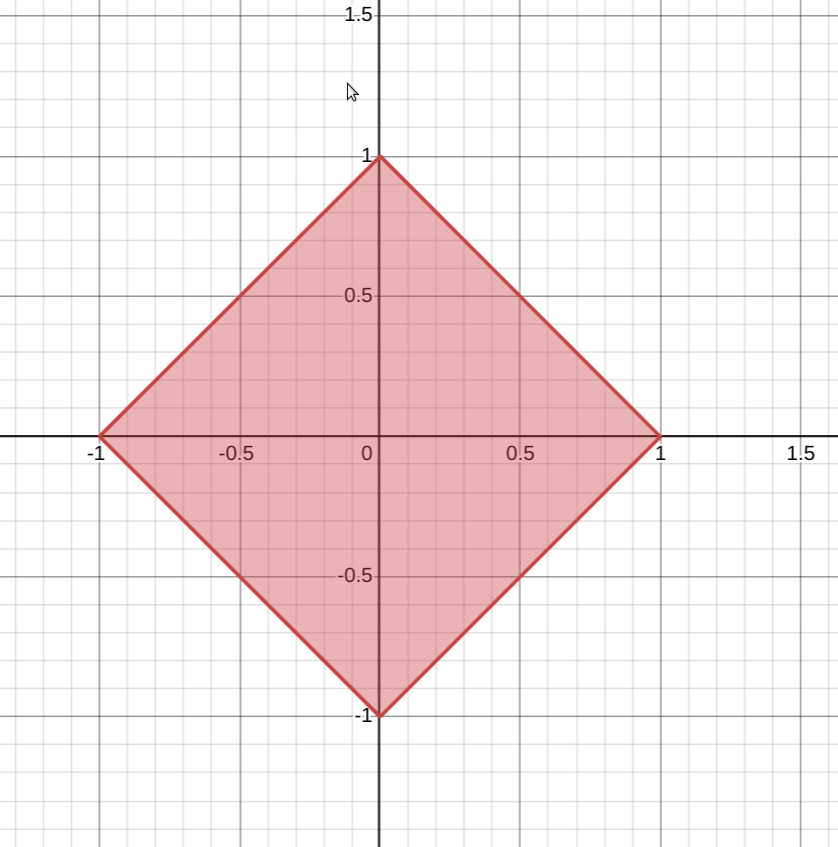
\includegraphics[width=0.3\textwidth]{unit-diamond.png}
                \end{figure}
            \item unit square centered at origin
                \begin{figure}[H]
                    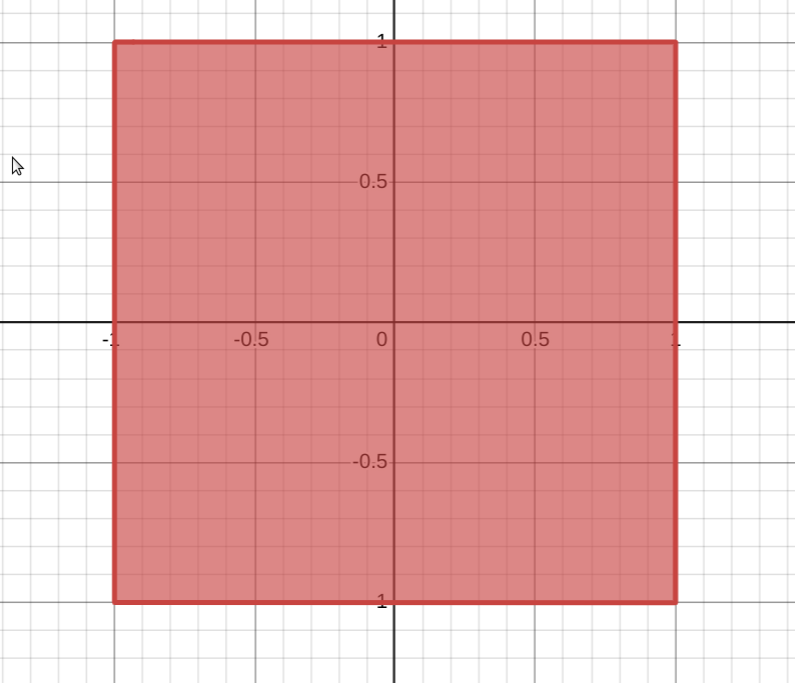
\includegraphics[width=0.3\textwidth]{unit_square.png}
                \end{figure}
        \end{enumerate}
    \item
        \begin{enumerate}
            \item     
        an eigenvector of a transformation $T : V \rightarrow V$ is a vector $v \in V$ such that $Tv = \lambda v$ for some $\lambda \in F$ where $F$ is the field.
        $\lambda$ is the eignevalue associated with the eigenvector $v$. an eigenvalue is any $\lambda \in F$ such that there exists $v \in V$ and $Tv = \lambda v$
        \item 
        \[
            (A - t I) = \begin{pmatrix} 2 - t & 1 \\ 1 & 2- t \end{pmatrix} \; \det (A-tI)  = (2-t)^2-1= 4 - 4t + t^2 -1 = 3 - 4t + t^2 = (t-1)(t-3)
        .\] 
        so $1,3$ are both eigenvalues. to find the eigenvectors we solve the following for non-trivial solution
        \[
            \begin{pmatrix} 1 & 1 \\ 1 & 1 \end{pmatrix} x = 0 \;\;\; x = \begin{pmatrix} a \\ -a \end{pmatrix}  
        .\] 
        for $\lambda = 1$
        and
        \[
            \begin{pmatrix} -1 & 1 \\ 1 & -1 \end{pmatrix}x = 0 \;\; x = \begin{pmatrix} a \\ a \end{pmatrix}
        .\] 
        for $\lambda = 3$
    \item clearly for every eigenvalue $\lambda_i$ of $A$ $\lambda_i^{k}$ is an eigenvalue of $A^{k}$. However the converse is not always true for 
        consider the transformation on $ \mathbb{R}^2$ by 
        \[
            A = \begin{pmatrix} 0 & -1 \\ 1 & 0 \end{pmatrix} 
        .\] 
            then $A$ has no eigenvectors or eigenvalues over $ \mathbb{R}$ but $A^2 = \begin{pmatrix} -1 & 0 \\ 0 & -1 \end{pmatrix} $ has
            eigenvectors with eigenvalue -1 of which $\sqrt{-1}$ is undefined so $-1$ is not $\lambda^2$ for some $\lambda \in \mathbb{R}$.
    \end{enumerate}
\item 
    \[
    a,x \in \mathbb{R}^{n} a^{T}x = a \cdot x = f
    .\] 
    If 
    \[
    a = \begin{pmatrix} a_1 \\ \vdots \\ a_d \end{pmatrix} , x = \begin{pmatrix} x_1 \\ \vdots \\ x_d \end{pmatrix} a^{T}x =  a_1 x_1 + \dots + a_d x_d  ,\;  \frac{df}{dx_i} = a_i \; \frac{df}{dx} = a
    .\] 
    \[
        A \in \mathbb{R}^{d \times d} = \begin{pmatrix} a_{11} & ... & a_{1d}\\ \vdots & \ddots & \vdots \\ a_{1d} & \dots & a_{dd} \end{pmatrix}  = \begin{pmatrix} A_1 & A_2 & \dots & A_d \end{pmatrix} 
    .\] 
    \[
        x^{T}Ax = \begin{pmatrix} \sum_{}^{}x_ia_{i 1} & \sum_{}^{}x_i a_{i 2}    & \dots & \sum_{}^{}x_i a_{i d} \end{pmatrix}x 
    .\] 
    \[
        = \sum_{j=1}^{d}x_j\sum_{i=1}^{d}x_ia_{ij} = \sum_{j=1}^{d}\sum_{i=1}^{d}x_ix_ja_{ij} = f
    .\] 
    \[
        \frac{df}{dx_i} = 2x_ia_{ii} + 2\sum_{j=1; j \ne i}^{d}x_ja_{ij} = 2\sum_{j=1}^{d}x_ja_{ji} = 2x^{T}A_{i}
    .\] 
    Additionally
    \[
        2\sum_{j=1}^{d}x_ja_{ji} = 2\sum_{j=1}^{d}a_{ij}x_j = 2(Ax)_i \implies \frac{df}{dx} = 2Ax
    .\] 
    then
    \[
        \frac{df}{dx_i} = 2x^{T}A_i = 2(\sum_{j=1}^{d}x_jA_{ji}) \implies \frac{d^2f}{dx_idx_j} = 2A_{ji} = 2A_{ij}
    .\] 
\item For any 2 $x_i,x_j$ such that $w^{T}x_i + b = 0$ and $w^{T}x_j + b = 0$
     \[
    \langle w, x_i - x_j \rangle = \langle w, x_i \rangle - \langle w, x_j \rangle = -b - (-b) = 0
    .\] 
    and so $w$ is orthogonal to the vector along the line defined by $w^{T}x + b$
    The distance from the origin to the line $w^{T}x + b = 0$ since letting $x = -\frac{b}{||w||^2}w$, we verify that
    \[
    \langle w, -\frac{b}{||w||^2}w \rangle = \frac{-b ||w||^2}{||w||^2} + b = -b + b = 0
    .\] 
    and so $x$ lies on the line. additionally, the vector is orthogonal to the line and so it represents the minimum distance to the line from the origin and its length is precisely.
    \[
    \sqrt{\langle -\frac{b}{||w||^2}w , -\frac{b}{||w||^2}w \rangle} = \sqrt{\frac{b^2}{||w||^{4}}||w||^{2}} = \sqrt{\frac{b^2}{||w||^2}} = \frac{b}{||w||}
    .\] 
    \end{enumerate}
}
\section{Problem 9}
\solution{
    \begin{enumerate}
        \item
             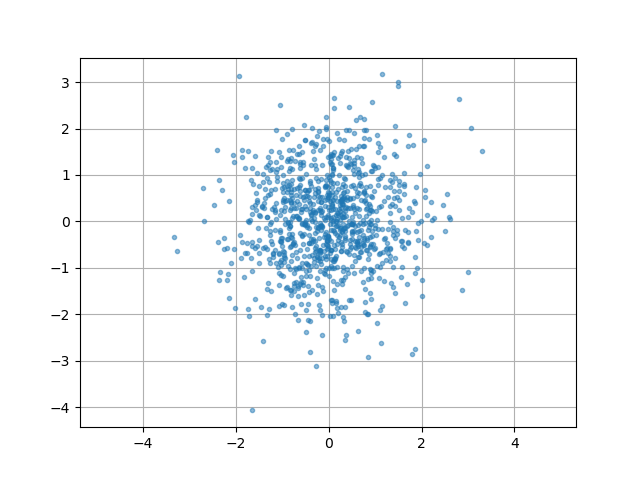
\includegraphics[width=0.3\textwidth]{9-a.png} 
        \item 
            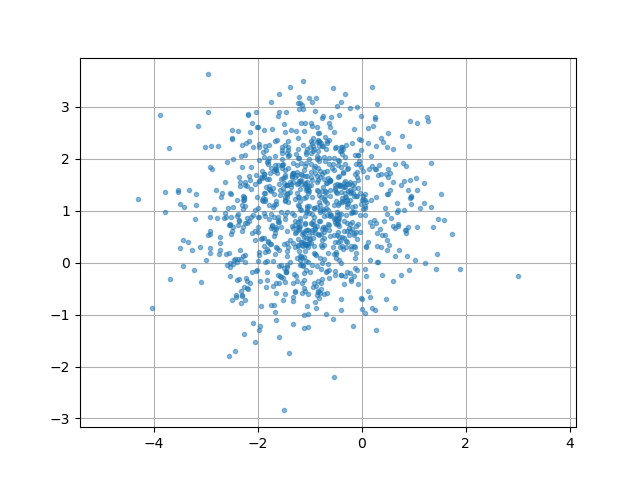
\includegraphics[width=0.3\textwidth]{9-b.png}
        \item 
            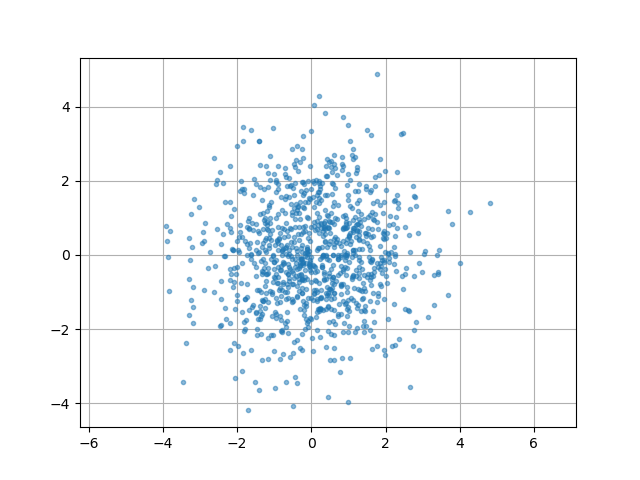
\includegraphics[width=0.3\textwidth]{9-c.png}
        \item 
            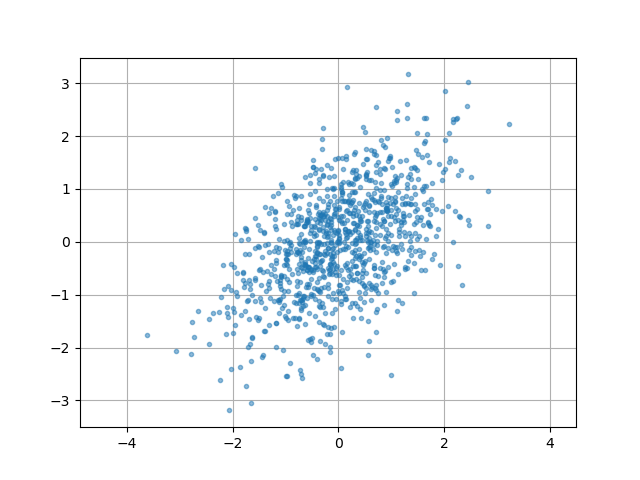
\includegraphics[width=0.3\textwidth]{9-d.png}
        \item
            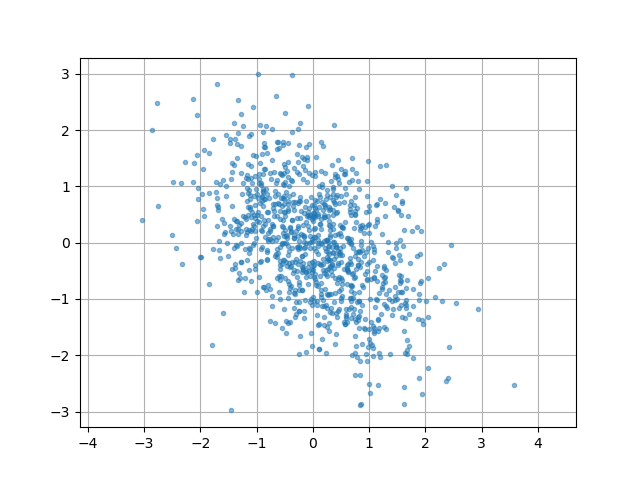
\includegraphics[width=0.3\textwidth]{9-e.png}
    \end{enumerate}
}
\section{Problem 10}
\begin{lstlisting}[language=Python]
import numpy as np
a = np.array(((1, 0),(1,3)))
values, vectors = np.linalg.eig(a)
i = np.argmax(values)
print(vectors[:,i])
\end{lstlisting}
\solution{
    outputs the vector $\begin{pmatrix} 0 \\ 1 \end{pmatrix} $ with eigenvalue $3$
}

\section{Problem 11}
 \solution{
     \begin{enumerate}
         \item The name of the data set is brain tumor datset
         \item the datset can be found at \url{https://figshare.com/articles/dataset/brain_tumor_dataset/1512427?file=51340418}
         \item The dataset includes images of tumors labeled as either mingioma, glioma, or pituitary tumor. As well as the images of the tumor and the pixel values where the tumor is located to train both 
             classification and for tasks such as finding the tumor in the picture (location).
         \item This dataset has 3064 images from 233 patients.
         \item each example has one feature (mingioma, glioma, or pituitary) and a number of features proportional to the number of pixels in the image
             as well as features indicating the border of the tumor.
     \end{enumerate}
 }
\end{document}
